\chapter{Realizacja projektu}

Praktyczną realizację projektu podzielono na dwie części. Pierwsza z nich dotyczyła zmian sprzętowych, koniecznych do zaimplementowania w robocie, natomiast druga część związana była z pracami programistycznymi jakie należało przeprowadzić. Poniżej dokładnie opisano cały proces.

\section{Prace sprzętowe}

W niniejszej sekcji przybliżono prace sprzętowe jakie wykonano nad robotem by móc go przystosować do tworzonego kontrolera. Manipulator, którym dysponowano po projekcie inżynierskim rozbudowano o dodatkowe mikrokontrolery oraz enkodery, tak by móc zaimplementować na nim docelowy kontroler ROS. 

\subsection{Montaż enkoderów}
Pierwszą kwestią jaką się zajęto związana była z zainstalowaniem enkoderów każdej osi.

Silniki krokowe wykorzystywane w robocie, w czasie swojej pracy wykonują jednostkowe kroki, przez co teoretycznie możliwe jest na tej podstawie stwierdzanie w jakim położeniu znajduje się dana oś robota. Można po prostu liczyć wykonane kroki. Teoretycznie takie rozwiązanie mogłoby być wystarczające w zbudowanym robocie, niemniej w zastosowaniach praktycznych raczej zawsze wykorzystuje się dodatkowe czujniki - enkodery. Pozwala to na mierzenie faktycznych ruchów poszczególnych osi. Oczywistym jest przecież, iż oś może być zablokowana bądź silnik po prostu zgubi kroki i przez to nie wykona żądanego odchylenia danego złącza. Tym samym informując kontroler o wykonaniu kroków, których tak naprawdę robot nie podjął, prowadzi to do sytuacji, kiedy to sterownik wykona planowanie w oparciu o błędne wskazania, a to przełoży się na dalsze przekłamania. Dysponując enkoderami kontroler będzie w stanie zgłosić błąd, jeśli ruch osi się nie odbył.


Zatem by sterownik robota mógł operować na faktycznych pomiarach przemieszczeń poszczególnych osi, postanowiono doposażyć robota w enkodery. Ze względu na różną specyfikę każdych złącz, w zależności od możliwości, montowano inne czujniki. Tak więc na części osi robota zamontowano enkodery REM5, natomiast na pozostałych posłużono się czujnikami szczelinowymi wraz z odpowiednio zamodelowanymi tarczami przysłonowymi. Pierwsze rozwiązanie jest znacznie dokładniejsze aniżeli to drugie, niemniej w żadnym przypadku rozdzielczość enkoderów nie jest mniejsza niż luz występujący na danym złączu (pomijając ramię główne, gdzie luz nie występuje). Jak wiadomo robot powstał w oparciu o metodę wydruku 3D, przez co przejawia pewne niedoskonałości, objawiające się chociażby wspomnianym luzem. 

O ile co do stosowania impulsatorów REM5 w odniesieniu do osi ramienia głównego, ramienia drugiego oraz trzeciego, nie było większych wątpliwości i trudności ich implementacji, o tyle długo zastosowano się nad obrotową wieżą. Ze względu na brak miejsca, nie było możliwości zamontowania enkodera na wale silnika, toteż zaproponowano poniższe rozwiązanie - rysunek \ref{fig:5}.

 \begin{figure}[H]
	\centering
	\includegraphics[width=0.9\linewidth]{{img/Bild_enkoder.jpg}}
	\caption{\centering Widok stworzonego enkodera obrotowej wieży oraz ramienia trzeciego. \cite{own}}
	\label{fig:5}
\end{figure}



Jak można zauważyć, do zliczania kątów odchyleń wieży, posłużono się dwoma czujnikami optycznymi umieszczonymi w specjalnie tym celu zamodelowanym mocowaniu. Przez szczeliny wspomnianych czujników przebiega swoista drabinka. Jest ona na stałe przymocowana do obrotowej wieży, natomiast czujniki optyczne do podstawy. Przez fakt, iż z punktu widzenia szczebli drabinki, czujniki są przesunięte względem siebie geometrycznie o kąt 90 stopni, sygnały jakie zwracają wraz z obracaniem wieży, to dwie przesunięte fale prostokątne. Uzyskano zatem klasyczny enkoder. W ten sposób możliwe jest zarówno zliczanie kątów jak i wyznaczanie kierunku ruchu.
Rozwiązanie to, mimo iż jego rozdzielczość jest mniejsza niż w przypadku pozostałych osi, to nadal jest bardziej precyzyjne, niż obecny na złączu naturalny luz.

Na rysunku \ref{fig:5} możliwe jest do zaobserwowania także mocowanie impulsatora REM5 do jednego z silników napędowych. We wszystkich pozostałych osiach, w których stosowano te enkodery wyglądało to podobnie, toteż już tego nie ilustrowano. Jako, iż enkodery te posiadają rozdzielczość 80 impulsów na obrót, to po uwzględnieniu przekładni napędzających je, otrzymywana dokładność jest znaczna. Dokładne zestawienie liczbowe zaprezentowano w  tabeli \ref{tab:3}.

Problematyczna okazała się także ostatnia z osi robota - obrót chwytaka. W tej sytuacji również nie było miejsca na zamontowanie enkodera REM5. Stwierdzono, iż ze względu na zastosowanie przekładni ślimakowej do jej napędzania - jej ruch możliwy jest jedynie włączając silnik napędowy. Z tego powodu zaproponowano poniższe rozwiązanie - rysunek \ref{fig:55}. 

 \begin{figure}[H]
	\centering
	\includegraphics[width=0.9\linewidth]{{img/Bild_enkoder_chwytak.jpg}}
	\caption{Widok enkodera osi obracającej chwytak. \cite{own}}
	\label{fig:55}
\end{figure}

Zainstalowany czujnik szczelinowy wraz z obrotem wału silnika wykrywa ruch tarczy przesłonowej, w wyniku czego możliwe jest liczenie impulsów przez mikrokontroler ESP8266. Natomiast kierunek ruchu ustalany jest na podstawie kierunku obrotu silnika. Jak wspominano nie ma innej możliwości poruszenia tąże osią, jak tylko włączając silnik. Samohamowność przekładni ślimakowej oraz miejsce umieszczenia wału silnika wewnątrz ramienia drugiego, niwelują możliwy wpływ czynników grawitacji i ingerencji użytkownika w ruch złącza.

Należy również nadmienić, iż podobnie jak to miało miejsce w przypadku projektowania całego manipulatora, tak i obecnie, w odniesieniu do wszelkich mocowań enkoderów, tarcz i drabinek przesłonowych - modelowanie tych elementów realizowano w programie Autodesk Inventor Professional 2021. Modele po wyeksportowaniu do formatu plików $.stl$ zamieniano na ciąg $.gcode$ w oprogramowaniu KISSlicer, a ostatecznie drukowano na drukarce Prusa i3 wyposażonej w otwartoźródłowe oprogramowanie Marlin. Stosowano filament PLA.

Poniżej w jednej tabeli zestawiono parametry wszystkich zainstalowanych enkoderów - tabela \ref{tab:3}

% Please add the following required packages to your document preamble:
% \usepackage[table,xcdraw]{xcolor}
% If you use beamer only pass "xcolor=table" option, i.e. \documentclass[xcolor=table]{beamer}
\begin{table}[H]
\caption{Zestawienie rozdzielczości poszczególnych enkoderów}
\label{tab:3}
\begin{tabular}{|c|c|c|
>{\columncolor[HTML]{C0C0C0}}c |c|
>{\columncolor[HTML]{C0C0C0}}c |ll}
\cline{1-6}
\cellcolor[HTML]{C0C0C0}L.p. & \cellcolor[HTML]{C0C0C0}Złącze         & \cellcolor[HTML]{C0C0C0}\begin{tabular}[c]{@{}c@{}}Rozdzielczość \\ enkodera {[}imp./obrót{]}\end{tabular} & \begin{tabular}[c]{@{}c@{}}Przekładnia\\ złącza\end{tabular} & \cellcolor[HTML]{C0C0C0}\begin{tabular}[c]{@{}c@{}}Rozdzielczość kątowa\\  złącza {[}°/obrót{]}\end{tabular} & \begin{tabular}[c]{@{}c@{}}Luz \\ złącza {[}st{]}\end{tabular} &  &  \\ \cline{1-6}
\cellcolor[HTML]{EFEFEF}1.   & \cellcolor[HTML]{EFEFEF}Obrót wieży    & \cellcolor[HTML]{EFEFEF}256                                                                                & \cellcolor[HTML]{EFEFEF}1                                    & \cellcolor[HTML]{EFEFEF}1° 24'                                                                               & \cellcolor[HTML]{EFEFEF}2° 50’                                 &  &  \\ \cline{1-6}
\cellcolor[HTML]{C0C0C0}2.   & \cellcolor[HTML]{C0C0C0}Ramię główne   & \cellcolor[HTML]{C0C0C0}80                                                                                 & 72                                                           & \cellcolor[HTML]{C0C0C0}0° 3' 45''                                                                           & Brak                                                           &  &  \\ \cline{1-6}
\cellcolor[HTML]{EFEFEF}3.   & \cellcolor[HTML]{EFEFEF}Ramię drugie   & \cellcolor[HTML]{EFEFEF}80                                                                                 & \cellcolor[HTML]{EFEFEF}14.0625                              & \cellcolor[HTML]{EFEFEF}0° 19' 12''                                                                          & \cellcolor[HTML]{EFEFEF}3° 05’                                 &  &  \\ \cline{1-6}
\cellcolor[HTML]{C0C0C0}4.   & \cellcolor[HTML]{C0C0C0}Ramię trzecie  & \cellcolor[HTML]{C0C0C0}80                                                                                 & 15                                                           & \cellcolor[HTML]{C0C0C0}0° 18' 0''                                                                           & 2° 41’                                                         &  &  \\ \cline{1-6}
\cellcolor[HTML]{EFEFEF}5.   & \cellcolor[HTML]{EFEFEF}Obrót chwytaka & \cellcolor[HTML]{EFEFEF}36                                                                                 & \cellcolor[HTML]{EFEFEF}25                                   & \cellcolor[HTML]{EFEFEF}0°  24' 0''                                                                          & \cellcolor[HTML]{EFEFEF}4° 3’                                  &  &  \\ \cline{1-6}
\end{tabular}
\end{table}

\subsection{Implementacja mikrokontrolera Raspberry Pi i ESP}

Enkodery należało oczywiście należycie podłączyć do mikrokontrolera, z którym współpracowały. W tym celu wykorzystano cienkie przewody pochodzące od przewodu Ethernetowego. Zasadniczo wszystkie czujniki robota łączono w ten sposób. Na końcach dolutowywano jeszcze wymagane zakończenia typu $goldpin$ - w zależności od potrzeb męskie bądź żeńskie.

Natomiast mikrokontroler STM32 był podłączony do sterowników silników krokowych jeszcze w ramach projektu inżynierskiego. Podobnie czujniki do bazowania, toteż nie było konieczności ingerencji w te elementy. Wystarczyło zatem sprząc STM32 z mikrokomputerem RPi4B z pomocą przewodu USB. 

Poniżej widok robota z profilu, przysposobionego w enkodery - rysunek \ref{fig:8}

 \begin{figure}[H]
	\centering
	\includegraphics[width=0.9\linewidth]{{img/Bild_unface.jpg}}
	\caption{\centering Widok robota z profilu. \cite{own}}
	\label{fig:8}
\end{figure}

Jak już możliwe jest do zaobserwowania - ilość przewodów biegnąca do roota jest znaczna. Jest to jeden z problemów jaki należałoby ewentualnie w przyszłości rozwiązać, gdyż przewody te stanowią utrudnienie w poruszaniu się manipulatora. Szczególnie niekorzystnie wpływają na możliwość jego obracania.

\section{Prace programistyczne}




\subsection{Oprogramowanie ESP - odczyt enkoderów}

Enkodery sprzężono z mikrokontrolerem ESP8266. Urządzenie to zaprogramowano napisanym kodem w języku C. Program wykorzystuje pseudosystem operacyjny FreeRTOS, na którym uruchomionych jest pięć osobnych wątków. Każdy wątek odpowiada za obsługę osobnego enkodera.

Pisanie oprogramowania na mikrokontroler ESP z wykorzystaniem $ESP8266\_RTOS\_SDK$ cechuje pewien narzucony schemat. Zatem w pierwszej kolejności niezbędne było określenie funkcji poszczególnych pinów. Wybrano toteż 9 możliwych do wykorzystania portów GPIO i określono ich funkcję jako piny wejściowe. Niestety 2 z używanych pinów pełnią istotną rolę przy starcie mikrokontrolera, przez co nie mogą przyjmować określonych stanów. Uwzględniając ten fakt, koniecznym jest odłączanie ich w momencie podłączania ESP do zasilania (podłączania przewodu USB do Raspberry Pi). 
W dalszej kolejności program inicjalizował wątki. Całość nie wykorzystuje systemu przerwań, jednak cyklicznie odczytuje stan każdego z podłączonych pinów. Każdy odczyt działa z okresem 10 milisekund.

Niestety enkodery nie są urządzeniami idealnymi. W związku z tym moment ich przełączania wiąże się z generacją swoistych drgań. Przejściu z jednego stanu do drugiego towarzyszą wielokrotne przełączenia wartości między tymi dwoma stanami. Jest to tak zwany $bouncing$. By program błędnie nie naliczał dodatkowych kroków wywołanych powyższym zjawiskiem zaimplementowano w programie prostą maszynę stanów zrealizowaną na instrukcji $switch$ języka C. Rozwiązanie to zupełnie rozwiązuje opisany problem. \cite{ESP_enc_file} 

Ostatnią kwestią było wysyłanie pomiarów przez port USB do mikrokomputera Raspberry Pi. Pierwotnie zakładano wysyłanie danych każdorazowo, po odnotowanej zmianie stanu danego enkodera. Niemniej później zrezygnowano z tego pomysłu, na rzecz stałej, synchronicznej wysyłki co 0.1 sekundy, bez względu na wystąpienie ruchu osi czy też nie. 

Poniżej widok  mikrokontrolera ESP8266 wraz z podpiętymi przewodami enkoderów - rysunek \ref{fig:6}. Poszczególne przewody zostały podpisane co ułatwiało późniejsze rozróżnienie ich.

 \begin{figure}[H]
	\centering
	\includegraphics[width=0.8\linewidth]{{img/Bild_ESP.jpg}}
	\caption{\centering Mikrokontroler ESP8266 wraz z podpiętymi przewodami enkoderów. \cite{ESP_enc_file}, \cite{own}}
	\label{fig:6}
\end{figure}

\subsection{Oprogramowanie Raspberry Pi}

Stworzony kontroler robota, tak jak to ukazano na poniższym rysunku \ref{fig:4}, zrealizowano w taki sposób, iż wszystkie najważniejsze obliczenia związane z planowaniem trasy realizowane są na laptopie, na którym też uruchomiony jest rdzeń ROSa (laptop pełni rolę mastera). Natomiast na mikrokontrolerze Raspberry Pi uruchamiano dwa węzły (node'y) ROSa. Jeden związany był z subskrybowaniem sygnałów sterujących pochodzących od plannera trajektorii. Węzeł ten wysyłał przeliczone ruchy poszczególnych złącz na ilości kroków do wykonania do mikrokontrolera STM, który to już sterował silnikami. Natomiast drugi węzeł - publisher wysyłał aktualne pozycje poszczególnych złącz z enkoderów. Informacje te otrzymywał z podłączonego poprzez port USB mikrokontrolera ESP8266. Subkryber i publisher uruchomione są jako dwa osobne wątki w programie napisanym w języku Python. Przy czym wątki te komunikują się ze sobą. \cite{Rasp_node_file}

%Realizując projekt zaproponowano niniejszą koncepcję połączenia poszczególnych elementów ze sobą - rysunek \ref{fig:4}

 \begin{figure}[H]
	\centering
	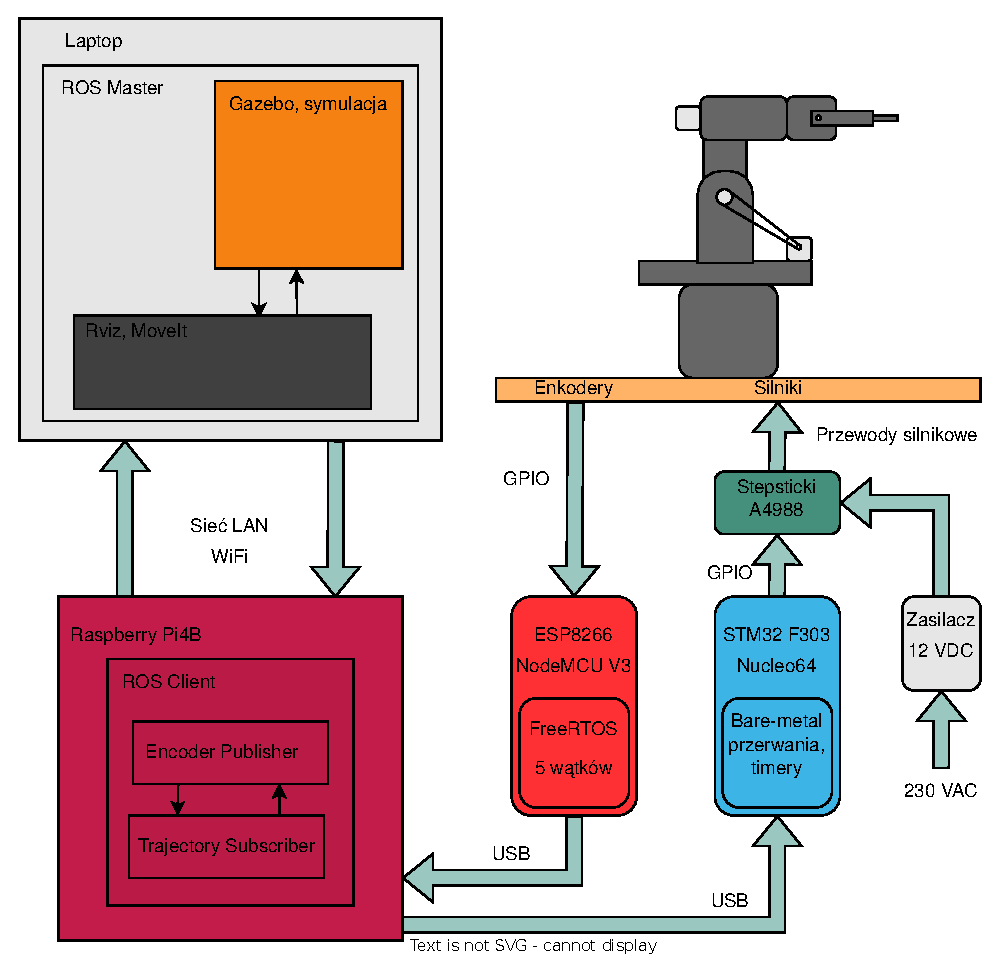
\includegraphics[width=0.9\linewidth]{{img/Bild_schemat.eps}}
	\caption{\centering Schemat połączeń poszczególnych elementów ze sobą. \cite{own}}
	\label{fig:4}
\end{figure}

Węzeł publikujący zrealizowano w taki sposób, iż w nieskończonej pętli "nasłuchuje" on wiadomości nadchodzących z ESP. Informacje te składają się z litery oraz liczby. Pierwsza litera informuje Raspberry Pi jakiego złącza dotyczy otrzymana wiadomość, natomiast liczba - o pozycji osi odczytanej z enkoderów. Węzeł ten synchronicznie publikuje wiadomości. Czyni to z częstotliwością 10 Hz do tematu $/joint\_state$.

Natomiast węzeł subskrybujący nasłuchuje wiadomości otrzymywanych od Mastera ROS (od laptopa). Dotyczy on tematu $/execute\_trajectory/goal$. Zatem w momencie otrzymania wiadomości wyciąga on z niej pozycje wszystkich złącz oraz ich prędkości. Następnie tłumaczy je na konkretne ilości kroków poszczególnych silników. Podobnie uwzględnia ich prędkość oraz kierunek ruchu. Ostatecznie formuje 32 znakową wiadomość, którą wysyła portem szeregowym do mikrokontrolera STM32. W niej zapisane są kierunki, prędkości oraz kroki do wykonania każdej osi. 

Przy czym istotne jest także, iż opisywany subskrybent rozróżnia sterowania dotyczące ramienia robota oraz samego chwytaka. Jeżeli kontroler ROS wysłał informację o ruchu chwytaka, wówczas wszystkie pola 32 znakowej ramki są zerami, z wyjątkiem dwóch ostatnich, gdzie subskrybent koduje informacje o nowej pozycji członu chwytającego.

iż w zależności czy sterowanie dotyczy ramienia robota czy samego chwytaka to subskrybent ten jest w stanie

Pisanie węzłów ROSa w języku Python dawało pewne ułatwienie aniżeli wykorzystując w tym celu język C++. Python nie wymaga kompilacji, jest językiem interpretowanym. W związku z tym napisany kod mógł być od razu uruchomiony instrukcją $rosrun$. Wszelkie publishery oraz subscribery napisane w C++ wymagałyby instrukcji $catkin$ $build$. Z kolei proces budowania, w momencie gdy aplikacja wykorzystywała liczne dodatkowe paczki ROSa, może być bardzo problematyczny do przeprowadzenia. Nierzadko pojawiają się liczne błędy związane z linkowaniem bibliotek, o których częściowo napisano w rozdziale 3.2.4. Dodatkowo gdy proces odbywa się na mikrokomputerze Raspberry Pi problemy te jedynie się nasilają.

Istotną kwestią, która zajęła sporo czasu był sam wybór systemu operacyjnego dla mikrokomputera Raspberry Pi. Sumarycznie przetestowano około 5 różnych systemów i dopiero ostatni spełniał wszystkie pożądane cechy - możliwe było na nim zainstalowanie ROSa Noetic oraz posiadał interfejs graficzny. Systemem tym okazał się Ubuntu Mate 20.04 przeznaczonym pod procesory ARM. Klasyczny Raspberry Pi OS nie posiadał w swoim repozytorium ROSa do zainstalowania, Ubuntu 22.04 pozwalało na zainstalowanie ROS, natomiast nie w dystrybucji Noetic, Ubuntu Server 20.04 pozwalał na zainstalowanie ROS Noetic, niemniej ze względu na brak interfejsu graficznego postanowiono go porzucić. Najprostsze podłączenie do sieci WiFi wiązało się wówczas z mozolnym wpisywaniem instrukcji do terminala. Pisanie jakiegokolwiek kodu w notatniku typu VIM nie jest optymalnym rozwiązaniem.


Jako iż robot posiada konstrukcję, w której silniki napędowe umieszczono w większości przy podstawie, toteż warunkuje to sposób zachowania się poszczególnych złącz urządzenia. Przede wszystkim poruszając ramieniem drugim manipulatora, porusza się jednocześnie obrotowa końcówka robota. Toteż chcąc utrzymać ją w niezmienionej pozycji, niezbędne jest kompensowanie ruchu ramienia drugiego, sterując również złączem ramienia trzeciego. Kompensację tę zrealizowano w sposób programowy i dlatego też oba węzły uruchamiane na mikrokomputerze Raspberry Pi komunikują się - tak by możliwe było kompensowanie wskazań enkoderów o ruchy związane z korektą pozycji niezbędną do utrzymania ramion zależnych od siebie w niezmienionej pozycji. Okazuje się iż znając między innymi przekładnie poszczególnych napędów osi można w precyzyjny sposób wyznaczyć tę kompensację.

Komunikacja między masterem uruchomionym na laptopie a ROSem pracującym na Rapberry Pi odbywała się przez Internet. Przy czym oba urządzenia musiały znajdować się w tej samej sieci lokalnej. W innym wypadku niezbędny musiałby być VPN, jednak rozwiązania tego nie testowano, gdyż nie było nawet takiej potrzeby. Niemniej możliwość taka istniała.

By komunikacja między urządzeniami zachodziła poprawnie niezbędne okazało się uruchomienie między nimi synchronizacji czasu, gdyż w przeciwnym wypadku ROS zgłaszał uwagi, iż pozycje poszczególnych złącz jakie otrzymuje są nieaktualne (różnią się stemplem czasowym). Dokładnie opisano to w kolejnych sekcjach.
\newpage

\subsection{Model robota w Gazebo}
\label{sub:ModelGazebo}

Jedną z wytycznych realizowanej pracy było przygotowanie wirtualnego modelu symulacyjnego z wykorzystaniem środowiska Gazebo. Model ten stworzono, w specjalnie w tym celu przygotowanym edytorze (będącego częścią pakietu Gazebo), do którego możliwe było załadowanie plików w formacie $.obj$ zawierających poszczególne osie robota. W ten sposób, kolejno dokładając następne fragmenty manipulatora zbudowano całe urządzenie. Dalej wyznaczono ruchome złącza dla każdej z osi i tym samym uzyskano gotowy model. Cały proces był dosyć intuicyjny, należało jedynie znać dobrze wymiary budowanego urządzenia, gdyż to w oparciu o nie dołączano kolejne fragmenty. Model ten wyeksportowano w dalszym kroku do pliku formatu $.sdf$ oraz $.config$, które posłużą dalej do wygenerowania pliku docelowego $.urdf$, wykorzystywanego przez ROSa, a dokładnie przez symulator Gazebo, jak i Rviz. \cite{URDF_file}

Gazebo również udostępnia możliwość tworzenia własnego świata, w którym zamierza się zainstalować posiadane urządzenie, niemniej z opcji tej nie korzystano. Postanowiono miast tego ręcznie zedytować model robota dokładając do niego jeszcze widniejące na poniższym rysunku \ref{fig:2} podstawę i stoliki. Elementy te są oczywiście uwzględniane przez plannery jako obiekty kolizyjne.

 \begin{figure}[H]
	\centering
	\includegraphics[width=0.9\linewidth]{{img/Bild_gazebo_2.png}}
	\caption{\centering Wirtualny model robota symulowany w środowisku Gazebo. \cite{own}, \cite{oak}, \cite{logo}}
	\label{fig:2}
\end{figure}

Plikiem opisującym importowane środowisko pracy robota, jest format $.world$. Zasadniczo korzystano z domyślnego pustego świata, niemniej na potrzeby późniejszych testów zmodyfikowano go nieco. Dodano niewielki obiekt - kostkę mydła na stoliku przed robotem. Jest ono widoczne na fotografii powyżej - rysunek \ref{fig:2}. \cite{seife_code}

W celu skonfigurowania modelu robota w ROSie posłużono się oprogramowaniem Setup Assistant. Jest to samodzielnie działający pakiet ROSa umożliwiający skonfigurowanie własnego robota i wygenerowanie wszystkich niezbędnych plików do symulowania oraz planowania trajektorii poruszania się manipulatora. Poniższe zdjęcie obrazuje omawiany program - rysunek \ref{fig:9}.

 \begin{figure}[H]
	\centering
	\includegraphics[width=0.9\linewidth]{{img/Bild_SA.png}}
	\caption{\centering Proces konfiguracji robota w programie MoveIt Setup Assistant. \cite{own}, \cite{oak}, \cite{logo}}
	\label{fig:9}
\end{figure}

Jak można zaobserwować z lewej strony powyższego rysunku \ref{fig:9} program ten pozwala na ustawienie wielu parametrów manipulatora. Ustawiono zatem kwestie wzajemnych kolizji jednych elementów robota z innymi. Całą konstrukcję podzielono na dwie grupy złącz. Pierwsza dotyczyła samego ramienia robota, natomiast druga - chwytaka. W dalszej kolejności ustalono charakterystyczne pozycje urządzenia. W tym przypadku pozycja określana jako $home$, to ta w której urządzenie znajduje się po bazowaniu. Zakładka $End$ $Effectors$ związana była z ustawieniami chwytaka - jakie złącza wchodzą w jego skład oraz które jest tak zwanym rodzicem chwytaka, czyli do którego członu jest on przymocowany.

Jedną z najistotniejszych zakładek stanowiła ta odpowiedzialna za konfigurację kontrolerów. To tutaj ustalono jaki planner wykorzystać i jakimi złączami ma sterować. Stworzono dwa kontrolery - jeden dla ramienia oraz drugi dla chwytaka.

Bardzo istotna była także zakładka kolejna, w której możliwe było wygenerowanie pliku $.urdf$ dla symulatora Gazebo.  Plik ten później jeszcze modyfikowano, gdyż dodano do niego fragmenty odpowiedzialne za określanie tekstur obiektów. Ważny jest tutaj fakt, iż Gazebo wymaga osobnych instrukcji opisujących tekstury obiektów aniżeli sam Rviz, który również wczytuje model robota. Toteż konieczne było dodanie fragmentów, które pozwoliły na ich uwzględnienie przez Gazebo. Na koniec wpisywano jeszcze informacje o autorze pracy i ostatecznie generowano automatycznie pliki.

Oczywiście wszystkie skrypty można pisać osobiście, jednak Setup Assistant czyni to znacznie szybciej i przede wszystkim zgodnie ze sztuką. Zatem generuje on niezbędne pliki uruchomieniowe (o rozszerzeniu $.launch$) oraz konfiguracyjne ($.yaml$).

\subsection{Uruchomienie i konfiguracja ROS i MoveIt}

Realizację całego projektu rozpoczęto od pobrania i zainstalowania ROSa. Proces ten należy przeprowadzi w zgodzie z oficjalną instrukcją. Jednak zanim to nastąpiło konieczne było zdecydowanie się na konkretną dystrybucję. W programie wykorzystano ROS Noetic, która jest rekomendowana. Decyzja wyboru dystrybucji nie mogła być bez znaczenia, gdyż występują paczki (specyficzne funkcjonalności), dostępne jedynie pod konkretne dystrybucje. Podobnie nie każda dystrybucja jest dostępna na każdy system operacyjny - było to szczególnie istotne w przypadku Raspberry Pi. Podobnie nie wszystkie dystrybucje wspierają MoveIt. 

Na laptopie, który miał z założenia pełnić role Mastera zainstalowano ROSa w pełnej wersji wraz ze wszystkimi pomocami graficznymi, takimi jak Rviz oraz RQT.


W pierwszej kolejności należało pobrać zawartość repozytorium oprogramowania ROS a następnie odpowiednio go zainstalować. Niezbędne było również dodanie do pliku $~/.bashrc$ informacji o lokalizacji ROSa, tak by otwierając nowe okno terminala, ROS był od razu widoczny.

Dodatek MoveIt zainstalowano z pomocą instrukcji $apt$ $install$, niemniej próbowano także zrealizować to przez tak zwaną instalację ze źródła. W momencie gdy docierano do procesu kompilowania paczek MoveIt pojawiały się liczne błędy. Budowanie udało się dokończyć dopiero na maszynie wirtualnej symulującej Ubuntu 20.04 z zainstalowanym ROSem Noetic. Problemy przy kompilacji jakichkolwiek paczek ROS wynikały z brakujących bibliotek w czasie linkowania, mimo iż biblioteki te były na komputerze zainstalowane. Powodem części niepowodzeń był jednak fakt, że niektórych z bibliotek było więcej (w różnych wersjach) i przez to linker zwracał błędy, nie wiedząc której z nich użyć. Mimo wszystko do końca realizowanego projektu nie udało się w pełni rozwiązać tych problemów, przez co wszystkie kompilacje prowadzono z poziomu dodatkowej maszyny wirtualnej. Jest to o tyle istotne, iż opisywane w poprzednim podrozdziale tworzenie modelu robota w programie Setup Asisstant po wygenerowaniu plików wymagało właśnie kompilacji.

%Tutaj również pojawiały się spore problemy, ze względu na fakt, iż oprogramowanie nie chciało się skompilować. Rzecz ta udała się dopiero na maszynie wirtualnej. W przypadku natywnie zainstalowanego ROS na komputerze osobistym kompilacja kończyła się niepowodzeniem, ze względu na obecne w systemie dwie biblioteki boost w różnych wersjach. Jako iż, biblioteki te były dwie, toteż kompilator 'nie wiedział', którą wybrać przez co zwracał błędy. 

Dysponując już całością koniecznego oprogramowania i stworzonym modelem, możliwe było uruchomienie programu Rviz wraz z dodatkiem MoveIt. Rezultat zaprezentowano poniżej - rysunek \ref{fig:3}.

Oczywiście Rviz nie jest wymagany do planowania i wykonywania trajektorii ruchu robota, gdyż jak to później zostanie przedstawione w rozdziale poświęconym testom, możliwe jest napisanie odpowiedniego skryptu, który zrealizuje to automatycznie. Niemniej wizualizuje on cały proces, co bardzo ułatwia jego zrozumienie. 

Wszystkie funkcje pakietu MoveIt, które można modyfikować z poziomu Rviza, obecne są w lewym dolnym rogu rysunku \ref{fig:3}.

 \begin{figure}[H]
	\centering
	\includegraphics[width=0.9\linewidth]{{img/Bild_rviz.png}}
	\caption{\centering Wirtualny model robota symulowany w środowisku Gazebo. \cite{own}, \cite{oak}, \cite{logo}}
	\label{fig:3}
\end{figure}

Ustalenie nowej pozycji, jaką żądano by robot osiągnął, można było dokonać na dwa sposoby. Pierwszym było poruszanie samym manipulatorem z pomocą widocznych na ramieniu trzecim kolorowych strzałek i pierścieni. Natomiast drugi sposób to ustalenie konkretnych pozycji złącz suwakami w zakładce $joints$.

Istotne jest w przypadku planowania trasy z pomocą MoveIt w programie Rviz zwracanie uwagi na punkt od którego trasa została wyznaczona. Za każdym razem należy wybierać opcję $current$, gdyż w przeciwnym wypadku planowanie nie odbędzie się od obecnej pozycji, tylko poprzedniej, co prowadzi później do niepożądanych sterowań. \cite{ROS_controller_file}

\subsection{Komunikacja zdalna i synchronizacja czasu}

Środowisko ROS umożliwia komunikację ze sobą i współpracę kilku urządzeń - znajdujących się w tej samej sieci lokalnej. Jest to szczególnie przydatne, gdyż moc obliczeniowa jednego komputera może nie być wystarczająca do uruchomienia symulacji np. Gazebo oraz pozostałej funkcjonalności. Stąd też powyższa funkcjonalność.

Autorowi projektu zależało by to komputer na którym jest uruchamiany rdzeń ROS-a, tzw. Master przejmował na siebie większość najważniejszych kwestii związanych chociażby z planowaniem oraz symulacją. Natomiast mikrokontroler Raspberry Pi4B stanowił jedynie łącznik, na który odbierał sygnały z Mastera i z pomocą portów USB komunikował się mikrokontrolerami wykonawczymi STM i ESP. Istniała co prawda możliwość sterowania stepstickami robota bezpośrednio z poziomu Raspberry, niemniej dla zabezpieczenia się przed ewentualnymi uszkodzeniami, pozostawiono STM32.

Przy czym kod źródłowy mikrokontrolera STM32 również wymagał wprowadzenia zmian, w związku z koniecznością odbierania wiadomości od RPi4B. Zatem jego oprogramowanie zmodyfikowano o odczyt z pomocą DMA informacji przychodzących z USB, po czym wyciąganie z nich zarówno prędkości każdego z silnika, jak i ilości kroków do wykonania. 

W celu uruchomienia ROSa na różnych urządzeniach wystarczy dokonać wpisu do pliku konfiguracyjnego $~/.bashrc$. Wystarczy dodać niniejszą instrukcję na komputerze Mastera:

\begin{minted}{bash}
# ~/.bashrc: executed by bash(1) for non-login shells.
# [...]
export ROS_MASTER_URI=http://192.168.0.103:11311 # IP laptopa
export ROS_IP=192.168.0.103 # IP laptopa
# [...]
\end{minted}

Oraz na pozostałych urządzeniach:

\begin{minted}{bash}
# ~/.bashrc: executed by bash(1) for non-login shells.
# [...]
export ROS_MASTER_URI=http://192.168.0.103:11311 # IP laptopa
export ROS_IP=192.168.0.101 # IP Raspberry Pi
# [...]
\end{minted}

Po sprzężeniu ze sobą komputera i Rasberry okazało się, iż niezbędne jest jeszcze uruchomienie synchronizacji między dwoma urządzeniami. W przeciwnym wypadku ROS zwracał ostrzeżenia o nieaktualnych pozycjach złącz. W tym celu uruchomiono na laptopie serwer czasu NTP, a na mikrokomputerze jego klienta. Skorzystano z protokołu Chrony. Po zainstalowaniu programu Chronyd na obu urządzeniach, niezbędne było przeprowadzenie konfiguracji systemu w plikach ustawieniowych ($/etc/chrony.conf $). W laptopie należało podać adres IP urządzeń, którym zezwala się podłączyć do synchronizatora czasu (wpis $allow$ $192.168.0.103$). Natomiast w RPi4B adres serwera (wpis $server$ $192.168.0.101$).

 \begin{figure}[H]
	\centering
	\includegraphics[width=1\linewidth]{{img/Bild_chrony.png}}
	\caption{ \centering Włączona synchronizacja czasu na Raspberry Pi. \cite{own}}
	\label{fig:46}
\end{figure}

Na obrazie powyżej ukazano terminal mikrokomputera Raspberry Pi z wywołaną komendą odpowiedzialną za wyświetlenie informacji na temat aktywnej synchronizacji czasu. Na pierwszej pozycji od góry tabeli widoczny jest adres laptopa, czyli przypisanego serwera. Podobnie laptop rozpoznaje podpiętych klientów - rysunek \ref{fig:47}{}

 \begin{figure}[H]
	\centering
	\includegraphics[width=1\linewidth]{{img/Bild_chrony_laptop.png}}
	\caption{ \centering Włączona synchronizacja czasu na laptopie. \cite{own}}
	\label{fig:47}
\end{figure}

Jak widać adres IP na obrazie ma końcówkę 104, co wynika z faktu, iż nie przypisywano temu Raspberry Pi stałego adresu, toteż czasami zmienia się on w zależności od ilości podpiętych do domowej sieci urządzeń.

Poniżej zaprezentowano (obraz \ref{fig:44}) proces testowania działania komunikacji między laptopem oraz Raspberry Pi. Na zdjęciu widoczny jest ekran laptopa na którym uruchomiono rdzeń ROS wraz z MoveItem w programie Rviz. Natomiast monitor wyświetla obraz z Raspberry Pi (widniejący ekran powitalny systemu Ubuntu Mate 20.04). W terminalach obu maszyn wywołano instrukcję $rostopic$ $list$, dzięki temu uzyskano potwierdzenie, iż komunikacja sieciowa działa. Dodatkowo na mikrokomputerze uruchomiono także program odpowiedzialny za wysyłanie stanu enkoderów, toteż widoczne jest, iż wirtualna pozycja robota odpowiada tej rzeczywistej.

 \begin{figure}[H]
	\centering
	\includegraphics[width=0.9\linewidth]{{img/Bild_all_robot.jpg}}
	\caption{ \centering Testy komunikacji między systemami i poprawności funkcjonowania enkoderów. \cite{own}, \cite{oak}}
	\label{fig:44}
\end{figure}

Na obrazie widoczny jest także sam mikrokomputer Raspberry Pi, w charakterystycznej, wydrukowanej czarnej obudowie z wentylatorem.

\section{Podsumowanie rozdziału}

Podsumowując zaprezentowane w niniejszym rozdziale prace można stwierdzić, iż realizowany projekt kontrolera był dosyć złożony. Wymagane były umiejętności w różnych dziedzinach. Wiele rzeczy realizowano po raz pierwszy przez co konieczne było zmaganie się z licznymi błędami. W czasie realizacji projektu uszkodzono także serwomotor odpowiedzialny za chwytak. Konieczna była jego wymiana. Podobnie awarii uległa karta pamięci w mikrokomputerze Raspberry Pi. Gdyby nie kopia projektu na repozytorium, wówczas cały program należałoby pisać od początku. Podobnie też wiele połączeń lutowanych musiano poprawiać, gdyż często się łamały pod wpływem ruchu robota bądź nie stykały jak powinny. Zatem wnioski jakie się nasuwają od strony technicznej to konieczność zabezpieczania swoich prac i bycia świadomym licznych niepowodzeń, a także zniszczeń.

Podobnie materiał z jakiego wydrukowano robota - PLA, źle znosi promieniowanie UV. Elementy robota, które w czasie realizacji projektu inżynierskiego pasowano ciasno na wcisk, okazywały się po czasie być luźne. Elementy minimalnie zmieniły swoje wymiary.

Realizacja projektu okraszona była także licznymi dodatkowymi zmianami i modyfikacjami, których jednak nie wymieniono w powyższym opisie. Często chęć zaimplementowania najprostszej funkcji wiązała się z wielogodzinnym poszukiwaniem rozwiązania, a zdarzały się sytuacje kiedy to po całym dniu okazywało się, iż dana funkcjonalność nie występuje.  
